\documentclass{standalone}
\standaloneconfig{border=10pt}
\usepackage[utf8]{inputenc}
\usepackage[french]{babel}
\usepackage{amsmath}
\usepackage{cases}
\usepackage{graphicx}
\usepackage{booktabs}

\begin{document}

\begin{minipage}{4.5in}
%\setlength{\parindent}{3pt}
%\setlength{\parskip}{3ex plus 0.5ex minus 0.2ex}

\textbf{\underline{Multiplexeur du micro-compteur}}
\begin{figure}
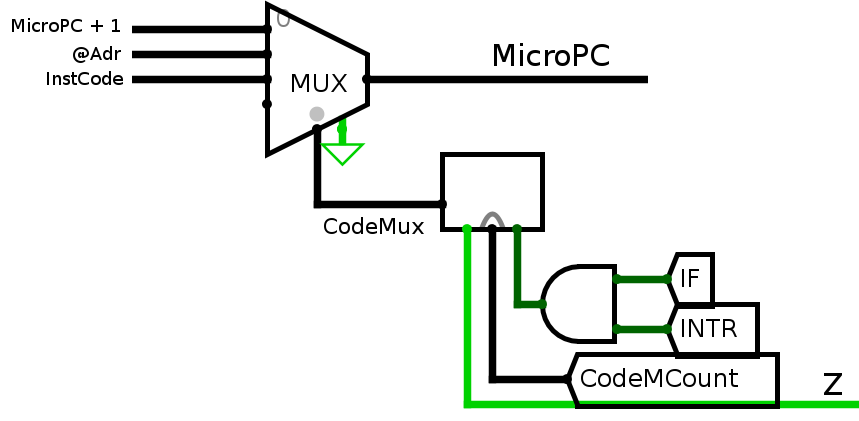
\includegraphics[width=0.5\textwidth]{mucount.png}
\end{figure}
\renewcommand{\arraystretch}{1.2}
\begin{tabular}{@{}lll||ll@{}}
\toprule
 CodeMCount & INTR\&IF & Z & CodeMux & Opération \\
\toprule
000 &  x & x & 00 & MicroPC := MicroPC + 1\\
001 &  x & x & 01 & MicroPC := @Adr\\
010 &  x & x & 10 & MicroPC := InstCode \\
011 &  x & 0 & 00 & MicroPC := MicroPC + 1 \\
011 &  x & 1 & 01 & MicroPC := @Adr \\
100 &  0 & x & 01 & MicroPC := @Adr \\
100 &  1 & x & 00 & MicroPC := MicroPC + 1 
\end{tabular}

\end{minipage}


\end{document}
